% --- CHUNK_METADATA_START ---
% src_checksum: 5e1f2c2ba1ee257dcb640b85c6873e4fc9406e761b51401dba246ca475b687d6
% needs_review: True
% --- CHUNK_METADATA_END ---
\chapter{Convergence in law}% --- CHUNK_METADATA_START ---
% src_checksum: e5d98871eb83d6fe24a2071cabd6ddf48b864f5993c60e49b2e8bc071dfd0d4e
% needs_review: True
% --- CHUNK_METADATA_END ---
\sloppy
The law is the most important thing.% --- CHUNK_METADATA_START ---
% src_checksum: d454e57a2ee4c97deb15b561528741158b313db7e80c38995edd92c632b4058c
% needs_review: True
% --- CHUNK_METADATA_END ---
\section{Definition}% --- CHUNK_METADATA_START ---
% src_checksum: 17cf386520b1cff0caee5c26fdda604d7a7ec0ceb86b0ef3dbafab97747d5be5
% needs_review: True
% --- CHUNK_METADATA_END ---
There exist sequences of random variables that converge neither almost surely, nor in probability, nor in $L^1$, yet whose distribution converges, or may even be constant.% --- CHUNK_METADATA_START ---
% src_checksum: 28c75232ace5ccdb780974a2b964b32646f5adfd5e07aaf88b8ce3b5ea0fda56
% needs_review: True
% --- CHUNK_METADATA_END ---
\begin{example}
Consider the probability space $(\Omega, \mathcal{F}, P) = ([0,1], \mathcal{B}([0,1]), \lambda)$ where $\lambda$ is the Lebesgue measure.
Consider the sequence of random variables $(X_n)$ defined for $\omega \in [0,1]$ by:
\begin{align*}
    X_{2n}(\omega) &= \mathbf{1}_{[0, 1/2]}(\omega) \\
    X_{2n+1}(\omega) &= \mathbf{1}_{[1/2, 1]}(\omega)
\end{align*}
This sequence converges neither almost surely, nor in $L^1$, nor in probability, but all the random variables follow the Bernoulli distribution with parameter $1/2$.
\begin{figure}[H]
    \centering
    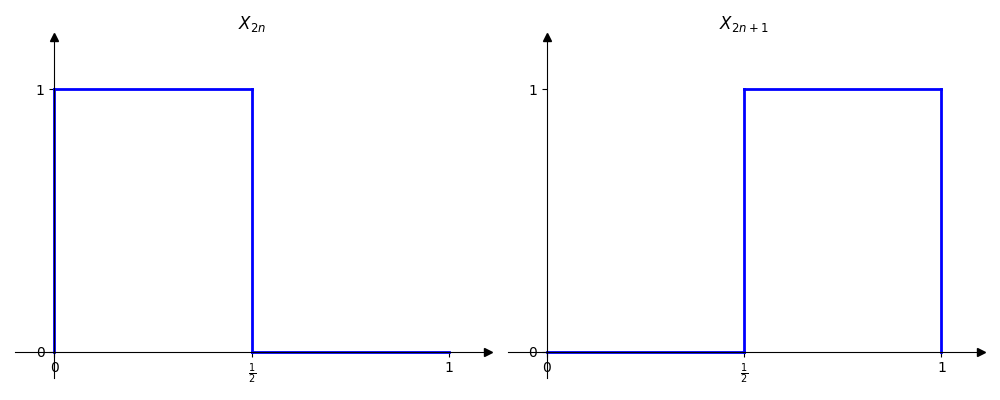
\includegraphics[width=0.6\textwidth]{convergence_en_loi_exemple.png}
    \caption{Representation of the random variables $X_{2n}$ and $X_{2n+1}$.}
    \label{fig:cv_loi_ex}
\end{figure}
For every $n$, the law of $X_n$ is the Bernoulli(1/2) distribution.
\[
\forall n, P(X_n=0) = P(X_n=1) = \frac{1}{2}
\]
and thus $P_{X_n} = \text{Ber}(1/2)$ does not depend on $n$.
\end{example}% --- CHUNK_METADATA_START ---
% src_checksum: 4abd4f1a873324b9fb96b499adec88c9c757837410a2f4356967f8dceecd9344
% needs_review: True
% --- CHUNK_METADATA_END ---
\begin{definition}[Convergence in Distribution]
Let $(X_n)_{n \in \mathbb{N}}$ be a sequence of real random variables (not necessarily defined on the same probability space). The sequence $(X_n)_{n \in \mathbb{N}}$ converges in law to a random variable $X$, denoted $X_n \xrightarrow{\mathcal{L}} X$, if and only if, for every bounded continuous function $f: \mathbb{R} \to \mathbb{R}$,
\[
\lim_{n \to \infty} \mathbb{E}[f(X_n)] = \mathbb{E}[f(X)].
\]
\end{definition}% --- CHUNK_METADATA_START ---
% src_checksum: 77616fade6cf57c0c556436d2b20a2371f536d2fa641b8afd9038d94efe8e37b
% needs_review: True
% --- CHUNK_METADATA_END ---

\begin{remark}
The expectation $\mathbb{E}[f(X_n)]$ depends only on the law of $X_n$, i.e.,
\[
\mathbb{E}[f(X_n)] = \int_{\Omega} f(X_n) dP = \int_{\mathbb{R}} f(x) dP_{X_n}(x).
\]
Thus, convergence in law applies even in situations where the random variables $X_n$ are not defined on the same probability space $(\Omega, \mathcal{F}, P)$, i.e., if $X_n: (\Omega_n, \mathcal{F}_n, P_n) \to (\mathbb{R}, \mathcal{B}(\mathbb{R}))$, where the $(\Omega_n, \mathcal{F}_n, P_n)$ have no a priori relation. This fundamentally distinguishes convergence in law from other modes of convergence.
\end{remark}
% --- CHUNK_METADATA_START ---
% src_checksum: 2aa52ad510726b3caef57cf7dc08a0b1aece75a005a487d1b046a605b928777b
% needs_review: True
% --- CHUNK_METADATA_END ---
\section{The cumulative distribution function}% --- CHUNK_METADATA_START ---
% src_checksum: 0fd1d09fe688835a7811b5ba9ae9b79ffd0148ffe592015e784ffe449070867b
% needs_review: True
% --- CHUNK_METADATA_END ---
A fundamental tool for studying probability laws on $\mathbb{R}$ is the cumulative distribution function.% --- CHUNK_METADATA_START ---
% src_checksum: 69b7896b87c071383ac06f0699bb04b77878efc12e065831f3d78b60417c5cfd
% needs_review: True
% --- CHUNK_METADATA_END ---
\begin{definition}
Let $X$ be a real-valued random variable defined on $(\Omega, \mathcal{F}, P)$. Its cumulative distribution function is the function $F_X$ defined by:
\[
\forall x \in \mathbb{R}, \quad F_X(x) = P(X \le x).
\]
We have $F_X(x) = P_X((-\infty, x])$. Since the intervals $(-\infty, x]$, $x \in \mathbb{R}$ generate the Borel sets and form a family stable under finite intersections, by the uniqueness of the $\pi$-$\pi-\lambda$ extension theorem, the law $P_X$ is determined by $F_X$.
Conclusion: the cumulative distribution function $F_X$ determines the law $P_X$ of $X$.
\end{definition}% --- CHUNK_METADATA_START ---
% src_checksum: 28bc179049e35ad42bd77738ed1a3eb0aa8c50c91058aad9e2f858f13fcf253c
% needs_review: True
% --- CHUNK_METADATA_END ---
A cumulative distribution function $F$ satisfies:% --- CHUNK_METADATA_START ---
% src_checksum: c7a8314d83a78c42d928db4101428719d050f741a62d16223afdf9933d9dde3e
% needs_review: True
% --- CHUNK_METADATA_END ---
\begin{enumerate}
    \item[i)] $F$ is increasing from $\mathbb{R}$ to $[0, 1]$.
    \item[ii)] $F$ is right-continuous at every point.
    \item[iii)] $\lim_{x \to -\infty} F(x) = 0$ and $\lim_{x \to +\infty} F(x) = 1$.
\end{enumerate}% --- CHUNK_METADATA_START ---
% src_checksum: 6d6cccf2cedc4fbe8626e53c0d0838b582e491f0815458ae183f373bed289eed
% needs_review: True
% --- CHUNK_METADATA_END ---
\begin{proof}
\begin{enumerate}
    \item[i)] By the increasing nature of the measure. If $x_1 \le x_2$, then $(-\infty, x_1] \subseteq (-\infty, x_2]$, so $P(X \le x_1) \le P(X \le x_2)$.
    \item[ii)] Let $x_0 \in \mathbb{R}$. Consider $\lim_{x \to x_0, x > x_0} F_X(x)$.
    Let $(x_n)_{n \in \mathbb{N}}$ be a sequence decreasing towards $x_0$. Then the sets $A_n = (-\infty, x_n]$ form a decreasing sequence of events. By monotone continuity of probability:
    \[
    \lim_{n \to \infty} F_X(x_n) = \lim_{n \to \infty} P(X \in A_n) = P(X \in \bigcap_{n=1}^\infty A_n) = P(X \in (-\infty, x_0]) = F_X(x_0).
    \]
    \item[iii)] By monotone continuity of probability. For the limit at $-\infty$, we take a sequence $x_n \to -\infty$ (e.g., $x_n=-n$).
    \[
    \lim_{x \to -\infty} F_X(x) = \lim_{n \to \infty} P(X \le -n) = P(\bigcap_{n=1}^\infty \{X \le -n\}) = P(\emptyset) = 0.
    \]
    For the limit at $+\infty$, we take a sequence $x_n \to +\infty$ (e.g., $x_n=n$).
    \[
    \lim_{x \to +\infty} F_X(x) = \lim_{n \to \infty} P(X \le n) = P(\bigcup_{n=1}^\infty \{X \le n\}) = P(X \in \mathbb{R}) = 1.
    \]
\end{enumerate}
\end{proof}% --- CHUNK_METADATA_START ---
% src_checksum: 3ff6055d5f1e157a6bcec7d8770616a134b0178f645c7288c588ca0a0fb74aaa
% needs_review: True
% --- CHUNK_METADATA_END ---
\begin{remark}
In some books, $F_X$ is defined as $F_X(x) = P(X < x)$. In this case, the distribution function is left-continuous.
\end{remark}% --- CHUNK_METADATA_START ---
% src_checksum: b0199b1f96f2eb30ba208c04466a4199f6dfbe3816045292147f699400eb581d
% needs_review: True
% --- CHUNK_METADATA_END ---
\begin{example}[Cumulative Distribution Functions of Standard Distributions]
\begin{enumerate}
    \item $X \sim \mathcal{B}(p)$ (Bernoulli distribution). $F_X(x) = 0$ if $x<0$, $1-p$ if $0 \le x < 1$, and $1$ if $x \ge 1$.
    \item $X \sim \mathcal{U}(\{1, \dots, n\})$ (Discrete uniform distribution). $F_X(x) = \frac{\lfloor x \rfloor}{n}$ for $1 \le x \le n$.
    \item $X \sim \mathcal{U}([0,1])$ (Continuous uniform distribution). $F_X(x) = 0$ if $x<0$, $x$ if $0 \le x \le 1$, and $1$ if $x>1$.
    \item $X \sim \text{Exp}(\lambda)$ (Exponential distribution). $F_X(x) = 1 - e^{-\lambda x}$ if $x \ge 0$, and $0$ if $x<0$.
    \item $X \sim \mathcal{N}(0,1)$ (Standard normal distribution). $F_X(x) = \int_{-\infty}^x \frac{1}{\sqrt{2\pi}} e^{-t^2/2} dt$.
\end{enumerate}
\begin{figure}[H]
    \centering
    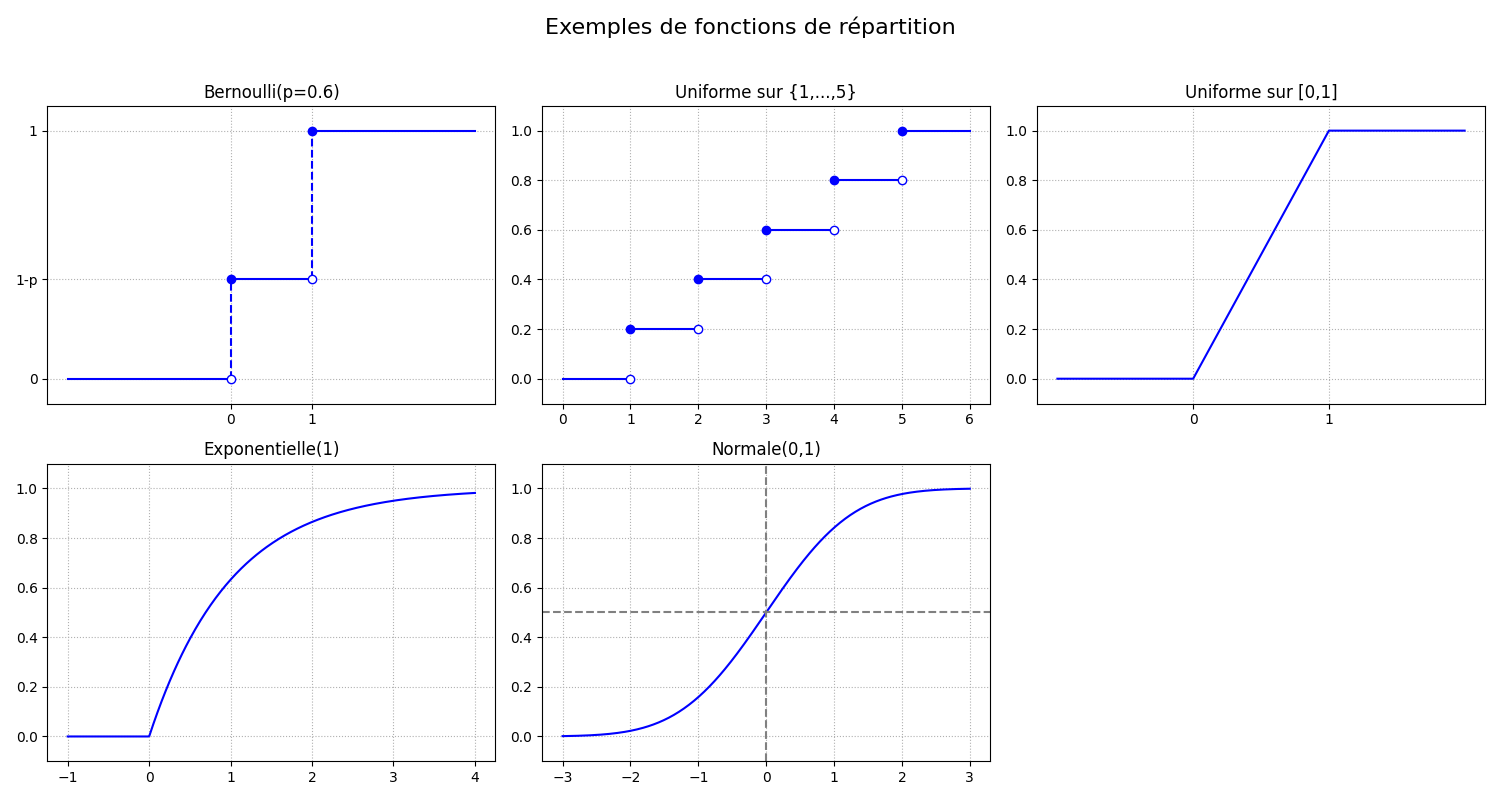
\includegraphics[width=\textwidth]{cdf_examples.png}
    \caption{Examples of cumulative distribution functions.}
    \label{fig:cdf_examples}
\end{figure}
\end{example}% --- CHUNK_METADATA_START ---
% src_checksum: 740408143e09e696f8cc7d6775b11295537d72422da6a5f90d85734d08b8d802
% needs_review: True
% --- CHUNK_METADATA_END ---
More generally, if the law of $X$ has a density $f$, then its cumulative distribution function is given by
\[
F_X(x) = \int_{-\infty}^x f(t) dt.
\]% --- CHUNK_METADATA_START ---
% src_checksum: be033d13426b0fceedbfb9b6d997a1e01e09eabaa1d860b943d0f0e3fd53a009
% needs_review: True
% --- CHUNK_METADATA_END ---
\begin{theorem}
Let $\mathcal{M}_1(\mathbb{R})$ denote the set of probability measures on $(\mathbb{R}, \mathcal{B}(\mathbb{R}))$, and let $\mathfrac{R}$ denote the set of functions satisfying the three properties of a distribution function. The mapping $\mu \mapsto F_\mu$, where $F_\mu(x) = \mu((-\infty, x])$, is a bijection from $\mathcal{M}_1(\mathbb{R})$ to $\mathfrac{R}$.
\end{theorem}% --- CHUNK_METADATA_START ---
% src_checksum: 208ebf83e6654019b6a7188439218366453a9a96eec1dfe5ec8ec4e1b207de3c
% needs_review: True
% --- CHUNK_METADATA_END ---
This is a difficult result, which in particular allows for the construction of singular probability measures on $(\mathbb{R}, \mathcal{B}(\mathbb{R}))$.% --- CHUNK_METADATA_START ---
% src_checksum: c8d62fa60a0bc39bd3a1aad1bd6b16bf26ea39b4352232d56ac41a3eaf6f9361
% needs_review: True
% --- CHUNK_METADATA_END ---
\begin{example}[Construction of a Singular Law]
One can construct a sequence of distribution functions $(F_n)$ on $[0,1]$ that converges uniformly to a continuous function $F_\infty$, the Cantor function. This function $F_\infty$ is a distribution function, but the associated probability measure $\mu$ is singular with respect to the Lebesgue measure $\lambda$. It has no atoms ($\mu(\{x\})=0$ for all $x$) and is concentrated on a set of Lebesgue measure zero (the Cantor set).

\begin{figure}[H]
    \centering
    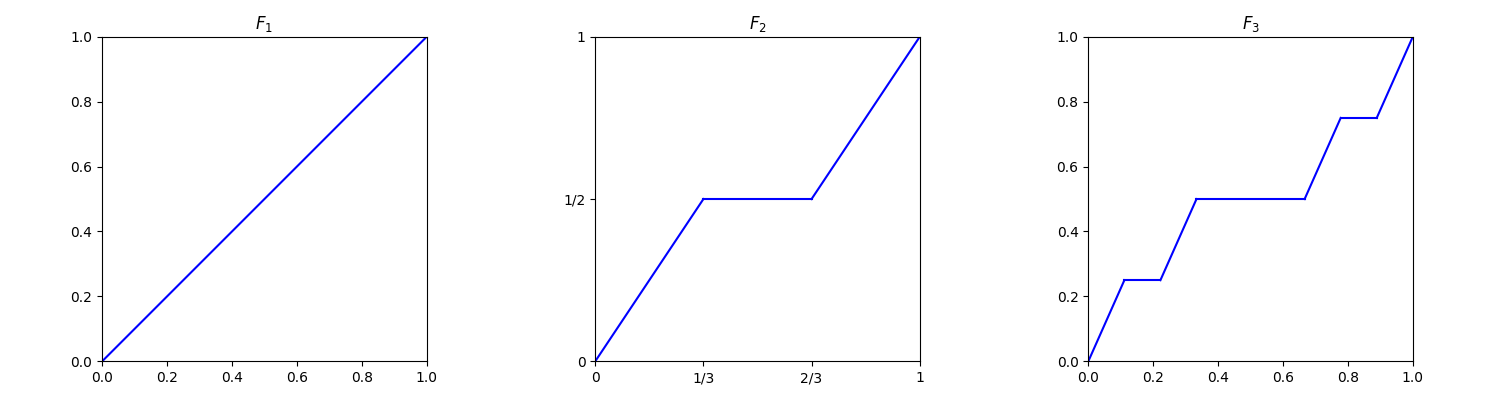
\includegraphics[width=0.8\textwidth]{cantor_construction.png}
    \caption{First steps in the construction of the Cantor function.}
    \label{fig:cantor}
\end{figure}
\end{example}% --- CHUNK_METADATA_START ---
% src_checksum: 8e922f868542c19deab220d229483a84e1a412fd4b29555836deb2f0c5cce6aa
% needs_review: True
% --- CHUNK_METADATA_END ---
\section{Convergence in law and cumulative distribution functions}% --- CHUNK_METADATA_START ---
% src_checksum: 70f2b1eb216bf98fdb1e37d8ab3fb0b1759fd9c12c718173341b248934c06763
% needs_review: True
% --- CHUNK_METADATA_END ---
Since convergence in law deals with the laws of random variables, it should be expressible via distribution functions.% --- CHUNK_METADATA_START ---
% src_checksum: 50e5485ffa7f570f5e55208611e0f03d165053cc481b247db7b66e7c249c0475
% needs_review: True
% --- CHUNK_METADATA_END ---
\begin{theorem}
Let $(X_n)_{n \in \mathbb{N}}$ be a sequence of real random variables and $X$ another real random variable. Let $(F_n)_{n \in \mathbb{N}}$ and $F$ be their corresponding cumulative distribution functions. The following statements are equivalent:
\begin{enumerate}
    \item[i)] The sequence $(X_n)$ converges in law to $X$ ($X_n \xrightarrow{\mathcal{L}} X$).
\item[ii)] At every point $x \in \mathbb{R}$ where $F$ is continuous, the sequence $(F_n(x))$ converges to $F(x)$, i.e., $\lim_{n \to \infty} F_n(x) = F(x)$.
\end{enumerate}
\end{theorem}% --- CHUNK_METADATA_START ---
% src_checksum: 25284f85b2547dd7506faf8d175c71f4a8b5d8fb11f3b0d1686714f574899fc1
% needs_review: True
% --- CHUNK_METADATA_END ---
\begin{proof}
$(i) \Rightarrow (ii)$: Let $x_0$ be a point where $F$ is continuous. We need to show that $\lim_{n \to \infty} F_n(x_0) = F(x_0)$.
For any $\epsilon > 0$, we can construct two bounded continuous functions $f_\epsilon$ and $g_\epsilon$ that "bound" the indicator function $\mathbf{1}_{(-\infty, x_0]}$ as follows:
\[
f_\epsilon \le \mathbf{1}_{(-\infty, x_0]} \le g_\epsilon
\]
such that $\mathbb{E}[g_\epsilon(X)] - \mathbb{E}[f_\epsilon(X)]$ is small.
For example, let $f_\epsilon$ be equal to 1 on $(-\infty, x_0-\epsilon]$, 0 on $[x_0, \infty)$ and linear in between.
Let $g_\epsilon$ be equal to 1 on $(-\infty, x_0]$, 0 on $[x_0+\epsilon, \infty)$ and linear in between.
\begin{figure}[H]
\centering
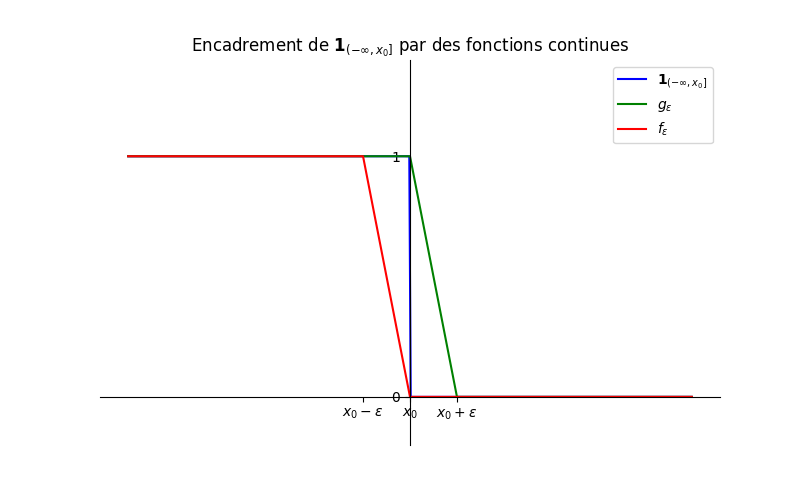
\includegraphics[width=0.6\textwidth]{sandwich_functions.png}
\caption{Functions $f_\epsilon$ and $g_\epsilon$ bounding $\mathbf{1}_{(-\infty, x_0]}$.}
\label{fig:sandwich}
\end{figure}
We have $f_\epsilon(y) \le \mathbf{1}_{(-\infty, x_0]}(y) \le g_\epsilon(y)$ for all $y \in \mathbb{R}$. Taking the expectation with respect to $X_n$:
\[
\mathbb{E}[f_\epsilon(X_n)] \le \mathbb{E}[\mathbf{1}_{(-\infty, x_0]}(X_n)] \le \mathbb{E}[g_\epsilon(X_n)]
\]
\[
\mathbb{E}[f_\epsilon(X_n)] \le F_n(x_0) \le \mathbb{E}[g_\epsilon(X_n)]
\]
Since $f_\epsilon$ and $g_\epsilon$ are continuous and bounded, and since $X_n \xrightarrow{\mathcal{L}} X$, we have:
\begin{align*}
    \lim_{n \to \infty} \mathbb{E}[f_\epsilon(X_n)] &= \mathbb{E}[f_\epsilon(X)] \\
    \lim_{n \to \infty} \mathbb{E}[g_\epsilon(X_n)] &= \mathbb{E}[g_\epsilon(X)]
\end{align*}
Taking the limit in the inequality, we obtain:
\[
\mathbb{E}[f_\epsilon(X)] \le \liminf_{n \to \infty} F_n(x_0) \le \limsup_{n \to \infty} F_n(x_0) \le \mathbb{E}[g_\epsilon(X)]
\]
Moreover, $\mathbb{E}[f_\epsilon(X)] \ge P(X \le x_0-\epsilon) = F(x_0-\epsilon)$ and $\mathbb{E}[g_\epsilon(X)] \le P(X \le x_0+\epsilon) = F(x_0+\epsilon)$.
Thus,
\[
F(x_0-\epsilon) \le \liminf_{n \to \infty} F_n(x_0) \le \limsup_{n \to \infty} F_n(x_0) \le F(x_0+\epsilon)
\]
Since $x_0$ is a continuity point of $F$, we have $\lim_{\epsilon \to 0} F(x_0-\epsilon) = \lim_{\epsilon \to 0} F(x_0+\epsilon) = F(x_0)$.
Taking $\epsilon$ to 0, by the squeeze theorem, we obtain:
\[
\lim_{n \to \infty} F_n(x_0) = F(x_0).
\]
$(ii) \Rightarrow (i)$:
Suppose that $F_{X_n}(x) \to F_X(x)$ at every point $x$ where $F_X$ is continuous. Let $f: \mathbb{R} \to \mathbb{R}$ be a continuous and bounded function. We need to show that $E[f(X_n)] \to E[f(X)]$.
Let $\epsilon > 0$. Since $\lim_{x \to -\infty} F_X(x) = 0$ and $\lim_{x \to +\infty} F_X(x) = 1$, there exist $a < b$, continuity points of $F_X$, such that $F_X(a) < \epsilon$ and $F_X(b) > 1-\epsilon$ (hence $P(X>b) < \epsilon$).
We decompose the expectation:
\[ E[f(X_n)] = \int_{x \le a} f(x) dP_{X_n} + \int_{a < x \le b} f(x) dP_{X_n} + \int_{x > b} f(x) dP_{X_n} \]
The integrals over the tails are small. For $n$ large enough, $F_{X_n}(a) \to F_X(a) < \epsilon$ and $1-F_{X_n}(b) \to 1-F_X(b) < \epsilon$.
\begin{align*}
    \left| \int_{x \le a} f(x) dP_{X_n} \right| &\le \|f\|_\infty P(X_n \le a) = \|f\|_\infty F_{X_n}(a) \xrightarrow{n \to \infty} \|f\|_\infty F_X(a) \le \epsilon \|f\|_\infty \\
    \left| \int_{x > b} f(x) dP_{X_n} \right| &\le \|f\|_\infty P(X_n > b) = \|f\|_\infty (1-F_{X_n}(b)) \xrightarrow{n \to \infty} \|f\|_\infty (1-F_X(b)) \le \epsilon \|f\|_\infty
\end{align*}
On the interval $[a,b]$, $f$ is uniformly continuous. It can be approximated by a step function. Let $a=x_0 < x_1 < \dots < x_k = b$ be a subdivision of continuity points of $F_X$. Define the step function $f_k^+$ by:
\[ f_k^+(x) = \sum_{l=1}^k \mathbf{1}_{]x_{l-1}, x_l]}(x) \sup_{t \in [x_{l-1}, x_l]} f(t) \]
Then $f(x) \le f_k^+(x)$ on $]a,b]$. We have
\[ \int_{a < x \le b} f(x) dP_{X_n} \le \int_{a < x \le b} f_k^+(x) dP_{X_n} = \sum_{l=1}^k \left( \sup_{t \in [x_{l-1}, x_l]} f(t) \right) (F_{X_n}(x_l) - F_{X_n}(x_{l-1})) \]
Taking the limit as $n \to \infty$, since the $x_l$ are continuity points:
\[ \limsup_{n \to \infty} \int_{a < x \le b} f(x) dP_{X_n} \le \sum_{l=1}^k \left( \sup_{t \in [x_{l-1}, x_l]} f(t) \right) (F_{X}(x_l) - F_{X}(x_{l-1})) = E[f_k^+(X)\mathbf{1}_{]a,b]}] \]
By uniform continuity of $f$ on $[a,b]$, as the subdivision step tends to 0 ($k \to \infty$), $f_k^+(x) \to f(x)$. By dominated convergence (since $|f_k^+| \le \|f\|_\infty$), we have $E[f_k^+(X)\mathbf{1}_{]a,b]}] \to E[f(X)\mathbf{1}_{]a,b]}]$.
Combining the bounds on the tails and the central interval, we obtain for arbitrarily small $\epsilon$ and sufficiently large $n$ and $k$:
\[ \limsup_{n \to \infty} E[f(X_n)] \le E[f(X)] \]
A similar argument with a lower bounding step function $f_k^-$ shows that:
\[ \liminf_{n \to \infty} E[f(X_n)] \ge E[f(X)] \]
We conclude that $\lim_{n \to \infty} E[f(X_n)] = E[f(X)]$.
\end{proof}